\chapter{Benchmark Design}
We developed a tool, called StreamBench, to execute benchmark workloads on stream processing systems. A key feature of StreamBench is extensibility, so that it could be extended not only to run new workloads but also to benchmark new stream processing systems. StreamBench is also available under an open source license, so that others may use and extend it, and contribute new workloads and stream processing system interfaces. We have used StreamBench to measure the performance of three selected stream processing systems, and that is reported in the next chapter.

This chapter illustrates the architecture of StreamBench and introduce more detail of main components of StreamBench. 

\section{Architecture}

\begin{figure}
  \begin{center}
  \subfigure{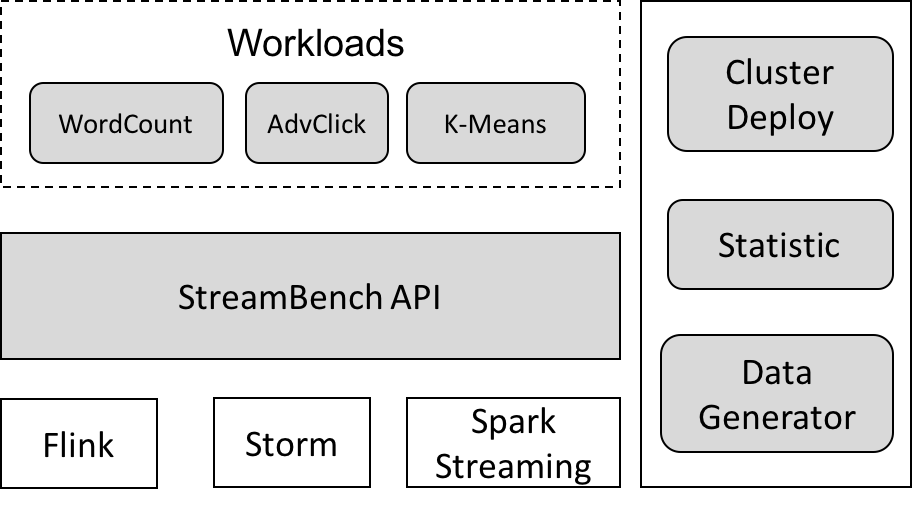
\includegraphics[scale=0.6]{images/benchmark_architecture}}
   \caption{StreamBench architecture}
   \label{fig:streambench_architecture}
  \end{center}
\end{figure}

The main component of StreamBench is a Java program for consuming data from partitioned kafka topic and executing workloads on stream processing cluster. The architecture of StreamBench is shown in Figure~\ref{fig:streambench_architecture}. The core of the architecture is StreamBench API which contains several states of stream and a set of stream processing APIs that are very similar to Flink's computational model. For example, API \texttt{mapToPair} maps a normal data stream to a keyed data stream, and API \texttt{filter} is a method with a parameter of boolean function and evaluates this boolean function for each element and retains those for which the function returns true. 

StreamBench API could be engined by different stream processing systems. Currently we support these APIs on three stream processing systems: Storm, Flink and Spark Streaming. It is very convenient to implement most interfaces of StreamBench API on Flink and Spark Streaming which have similar high level APIs. But there are also some APIs that Flink and/or Spark Streaming doesn't support well. For example, currently, Flink \texttt{join} operator only supports two streams joining on the same size window time. Therefore, we implemented another version \texttt{join} operator discussed in ~\cref{sub:join_operator} with Flink's low level API. Compare to Flink and Spark Streaming, Storm is more flexible by providing two low level APIs: spout and bolt. Bolts represent the processing logic unit in Storm. One can utilize bolts to do any kind of processing such as filtering, aggregating, joining, interacting with data stores, and talking to external systems.

With these common stream processing APIs, we implemented three workloads to benchmark performance of stream processing systems in different aspects. WordCount discussed in~\cref{sub:basic_operator} aims to evaluate the performance of stream processing systems performing basic operators. In~\cref{sub:join_operator}, we demonstrated a workload named AdvClick to benchmark two keyed streams joining operation. To check the performance of iterate operator, we designed a workload to calculate k-means of a point stream. More detail of this workload could be found in~\cref{sub:iterate_operator}.

Besides the core Java program, the architecture also includes three more components: Cluster Deploy, Data Generator and Statistic. Section~\ref{chapter:environment_setup} illustrates how to use cluster deploy scripts to setup experiment environment. Data generators generate test data for workloads and send it to kafka cluster that is demonstrated detailedly in ~\cref{section:data_generator}. The Statistic component discussed in ~\cref{section:log_statistic} includes experiment logging and performance statistic. 


\section{Experiment Environment Setup}
\label{chapter:environment_setup}

The experiment environment is a cloud service called cPouta which is the main production IaaS cloud at CSC -- a non-profit, state-owned company administered by the Ministry of Education and Culture. In cPouta,  there are several available virtual machine flavors. Each visual machine used in our experiment has 4 CPU cores, 15GB RAM, 10GB root disk and 220GB ephemeral disk. The experiment environment consists of two clusters: compute cluster and Kafka cluster. Computer cluster consists of 8 work nodes and one master nodes. Kafka cluster has 5 brokers with one zookeeper instance running on the same machine with one Kafka broker. The cPouta service is based on the hardware of the Taito cluster. Communication among nodes and to the storage is done by Infiniband FDR fabric, which provides low latency and high throughput connectivity. The detail information about hardware and inter connection could be found online~\footnote{\url{https://research.csc.fi/taito-supercluster\#1.1.2}}.

The operating system running on experiment nodes is Ubuntu 14.04 LTS. Benchmarked stream processing systems are Spark-1.5.1, Storm-0.10.0 and Flink-0.10.1. To enable checkpoint feature of Spark, Hadoop2.6(HDFS) is installed in compute cluster. Kafka 0.8.2.1 is running as distribute message system here. 

To deploy these software in compute cluster and kafka cluster automatically, we developed a set of python script. The prerequisites of using these scripts include internet access, ssh passwordless login between nodes in cluster and cluster configuration that describes which nodes are compute node or kafka node and where is the master node. The basic logic of deploy scripts is to download softwares online and install them, then replace configure files which are contained in a Github repository. For detail information of how to use cluster deploy scripts and configure of Storm, Flink, Spark and Kafka, please check this Github repository~\footnote{\url{https://github.com/wangyangjun/StreamBench}}.

\section{Workloads}
\label{section:workloads}

In StreamBench, a workload consists of a stream processing application and one or more kafka topics. The application consumes messages from kafka cluster and executes operations or transformations on the messages. We have developed 3 workloads to evaluate different aspects of a stream processing system. Each workload contains a representative operation or feature of stream processing system that can be used to evaluate systems at one particular point in the performance space. We have not attempted to exhaustively examine the entire performance space. As StreamBench is open sourced, users could also defined their own workloads either by defining a new set of workload parameters, or if necessary by implement a new workload which is discussed detailedly in~\cref{section:extensibility}.


\subsection{Basic Operators}
\label{sub:basic_operator}

With the widespread use of computer technologies, there is an increasing demand of processing unbounded, continuous input streams. In most cases, only basic operations need to be performed on the data streams such as \texttt{map}, and \texttt{reduce}. One good sample is stream WordCount. WordCount is a very common sample application of Hadoop MapReduce that counts the number of occurrences of each word in a given input set \cite{MapReduce}. Similarly, many stream processing systems also support it as an sample application to count words in a  given input stream. Stream WordCount is implemented with basic operations which are supported by almost all stream processing systems. It means either the system has such operations by default or the operations could be implemented with provided built-in APIs. Other basic operations include \texttt{flatMap}, \texttt{mapToPair} and \texttt{filter} which are similar to \texttt{map} and could be implemented by specializing \texttt{map} if not supported by default. The pseudocode of WordCount implemented with StreamBench APIs could be abstracted as Algorithm~\ref{alg:word_count}.

\begin{algorithm}
\caption{WordCount}\label{euclid}
\label{alg:word_count}
\begin{algorithmic}[1]
\State $\textit{sentenceStream.flatMap(...)}$
\State \hspace{2.6cm} $\textit{.mapToPair(...)}$
\State \hspace{2.6cm} $\textit{.reduceByKey(...)}$
\State \hspace{2.6cm} $\textit{.updateStateByKey(...)}$

\end{algorithmic}
\end{algorithm}

One special case of the basic APIs is \texttt{updateStateByKey}. Only in Spark Streaming there is a corresponding built-in operation. As discussed in Section~\ref{section:spark}, the computing model of Spark Streaming is micro-batch which is different with that of other stream processing systems. The results of operation \texttt{reduceByKey} of WordCount running in Spark Streaming is word counts of one single micro batch data set. Operation \texttt{updateStateByKey} is used to accumulate word counts in Spark Streaming. Because the model of Flink and Storm is stream processing and accumulated word counts are returned from \texttt{reduceByKey} directly. Therefore, when implementing the API \texttt{updateStateByKey} with Flink and Storm engine, nothing need to do. 

% window pre-aggregation
When dealing with skewed data, the compute node which count the word with largest frequency might be the bottleneck. Inspired from MapReduce Combiner, we designed another version of WordCount with \texttt{window} operator of stream processing. Windows are typically groups of events within a certain time period. In the reduce step of Windowed WordCount, first words are shuffle grouped and applied pre-aggregation. In a certain time period, local pre-aggregation results are stored at local compute nodes. At the end of a window time, the intermedia word counts are key grouped and reduced to get the final results.

%The goal of this workload is to evaluate the performance of stream processing systems executing basic operations.  
\begin{figure}
  \begin{center}
  \subfigure{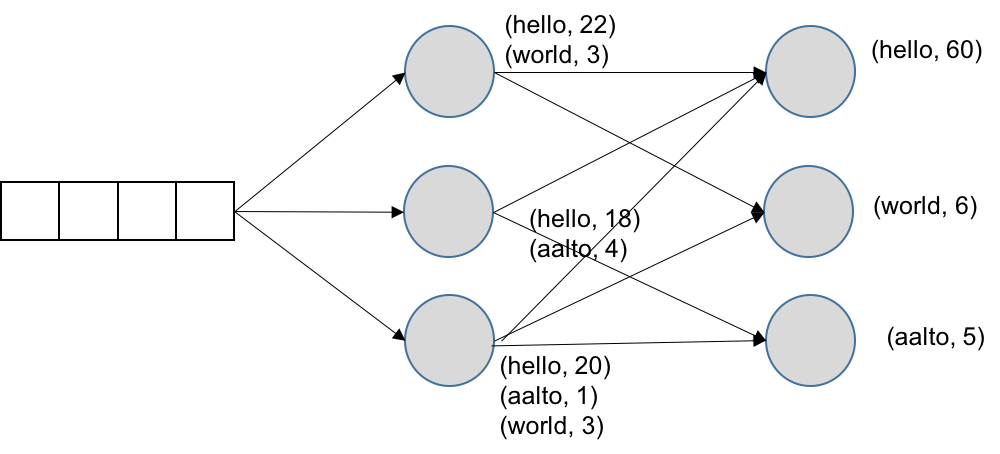
\includegraphics[scale=0.4]{images/window_wordcount}}
   \caption{Windowed WordCount}
   \label{fig:windowed_wordcount}
  \end{center}
\end{figure}


\subsection{Join Operator}
\label{sub:join_operator}

Besides the cases in which only basic operations are performed, another typical type of stream use case is processing joins over two input streams. For example, in a surveillance application, we may want to correlate cell phone traffic with email traffic. Theoretically unbounded memory is required to processing join over unbounded input streams, since every record in one infinite stream must be compared with every record in the other. Obviously, this is not practical\cite{window-join}. Since the memory of a machine is limited, we need restrict the number of records stored for each stream with a time window. 

A window join takes two key-value pair streams, say stream \textit{S1} and stream \textit{S2}, along with windows with the same slide size for both \textit{S1} and \textit{S2} as input. Each record in \textit{S1} is a tuple of pair \texttt{(k, v1)} with \texttt{k} as the primary key. The key in Stream \textit{S2:}\texttt{(k, v2)} is a foreign key referencing primary key in \textit{S1}. The output of join operator is a stream of tuple \texttt{(k, v1, v2)}. This primary key join operation could be described as a SQL query illustrated in Algorithm~\ref{alg:join_query}. Assuming a sliding window join between stream \textit{S1} and stream \textit{S2}, a new tuple arrival from stream \textit{S2}, then a summary of steps to preform join is the following:

\begin{algorithm}
\caption{Join Query}\label{euclid}
\label{alg:join_query}
\begin{algorithmic}[1]
\State SELECT $\textit{S1.k},  $\textit{ S1.v1},  $\textit{S2.v2}$
\State FROM $\textit{S1}$
\State INNER JOIN $\textit{S2}$
\State ON $\textit{S1.k}$ =  $\textit{S2.k}$
\end{algorithmic}
\end{algorithm}

\begin{enumerate}
\item Scan window of stream \textit{S1} to find any tuple which has the same key with this new tuple and propagate the result;
\item 
\begin{enumerate}
\item Invalidate target tuple in stream \textit{S1}'s window if found ;
\item If not, insert the new tuple into stream \textit{S2}'s window 
\end{enumerate}
\item Invalidate all expired tuples in stream \textit{S2}'s window.
\end{enumerate}

\begin{figure}
  \begin{center}
  \subfigure{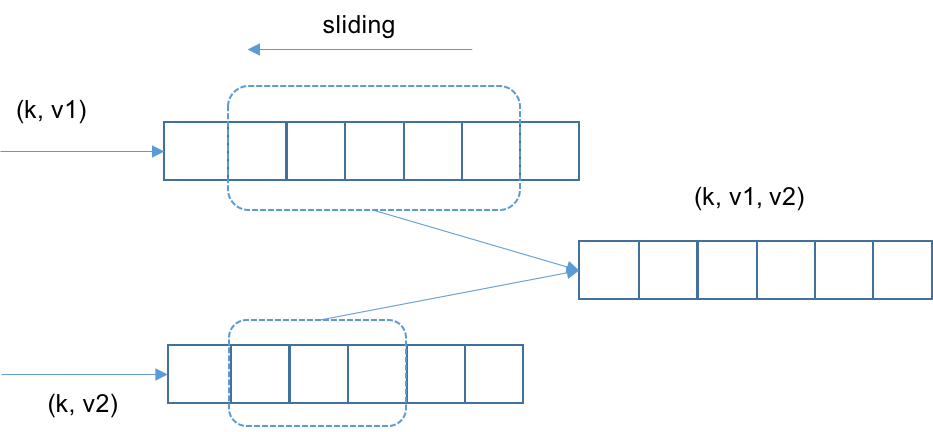
\includegraphics[scale=0.6]{images/join}}
   \caption{Window join scenario}
   \label{fig:window_join}
  \end{center}
\end{figure}

Every time new tuple arrives stream \textit{S2}, window of stream \textit{S1} need be scanned. That reduces the performance of join operation, especially when the window is big. With a data structure named \texttt{cachedHashTable} there is another way to implement stream join. The tuples in the window of a stream are stored in a cached hash table. Each tuple is cached for window time and expired tuples are invalidated automatically. One of such a \texttt{cachedHashTable} could be found in Guava.\footnote{\url{http://docs.guava-libraries.googlecode.com/git/javadoc/com/google/common/cache/CacheBuilder.html}} Instead of scanning window of stream \textit{S2}, we could find tuple with the same key in \textit{S2} directly by calling \texttt{cachedHashTable.get(k)}. In theory, this implementation achieves better performance. 

Since Spark Streaming doesn't process tuples in a stream one by one, the join operator in Spark Streaming has different behaviours. In each batch interval, the RDD generated by stream1 will be joined with the RDD generated by stream2. For windowed streams, as long as slide durations of two windowed streams are the same, in each slide duration, the RDDs generated by two windowed streams will be joined. Because of this, window join in Spark Streaming could only make sure that a tuple in one stream will always be joined with corresponding tuple in the other stream that arrived earlier up to a configureable window time. Otherwise, repeat joined tuples would exist in generated RDDs of joined stream. As Figure~\ref{fig:spark_join_norepeat} shown, a tuple in Stream2 could be always joined with a corresponding tuple in Stream1 that arrived up to 2 seconds earlier. Since the slide duration of Stream2 is equal to its window size, no repeat joined tuple exists. On the other hand, it is possible that a tuple arrives earlier from Stream2 than the corresponding tuple in Stream1 couldn't be joined. Figure~\ref{fig:spark_join_repeat} exemplifies that there are tuples joined repeatedly  when slide duration of Stream2 is not equal to its window size.

\begin{figure}
  \begin{center}
  \subfigure{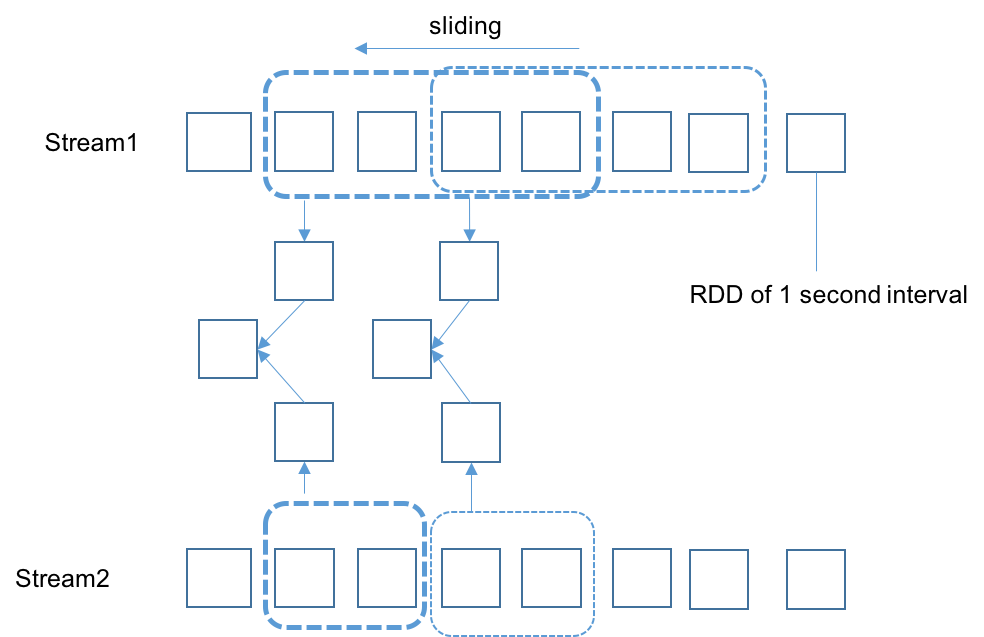
\includegraphics[scale=0.6]{images/spark_join_norepeat}}
   \caption{Spark Stream join without repeated tuple}
   \label{fig:spark_join_norepeat}
  \end{center}
\end{figure}


To evaluate performance of join operator in stream processing systems, we designed a workload called AdvClick which joins two streams in a online advertisement system. Every second there are a huge number of web pages opened which contain advertisement slots. A corresponding stream of shown advertisements is generated in the system. Each record in the stream could be simply described as a tuple of \texttt{(id, shown time)}. Some of advertisements would be clicked by users and clicked advertisements is a stream which could be abstracted as a unbounded tuples of \texttt{(id, clicked time)}. Normally, if an advertisement is attractive to a user, the user would click it in a short time after it is shown. We call such a click of an attractive advertisement valid click. To bill a customer, we need count all valid clicks regularly for advertisements of this customer. That could be counted after joining stream \texttt{advertisement clicks} and stream \texttt{shown advertisements}. 

\begin{figure}
  \begin{center}
  \subfigure{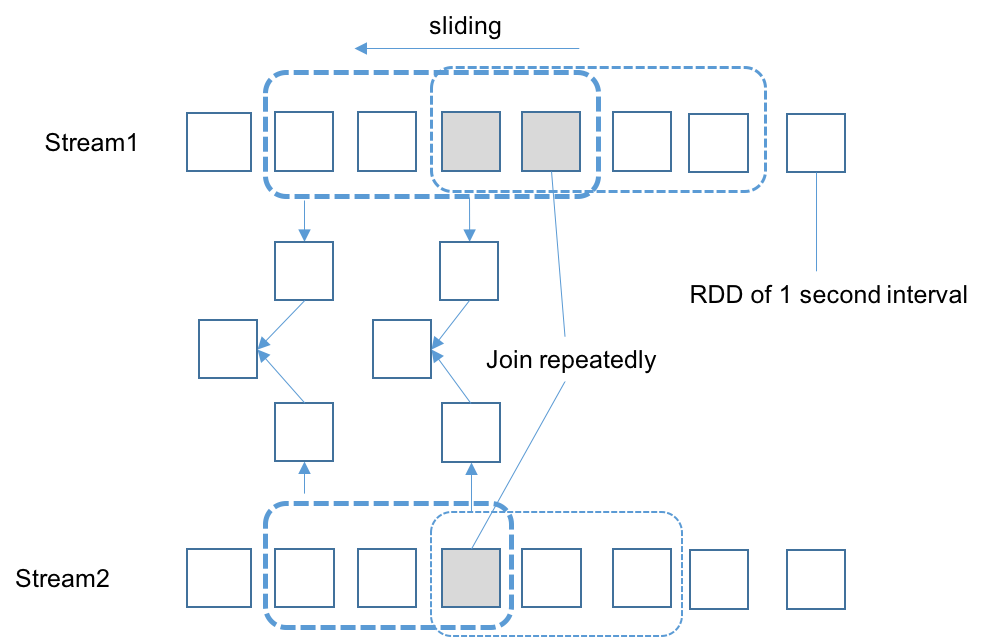
\includegraphics[scale=0.6]{images/spark_join_repeat}}
   \caption{Spark Stream join with repeated tuples}
   \label{fig:spark_join_repeat}
  \end{center}
\end{figure}

\subsection{Iterate Operator}
\label{sub:iterate_operator}

Iterative algorithms occur in many domains of data analysis, such as machine learning or graph analysis. Many stream data processing tasks require iterative sub-computations as well. These require a data processing system having the capacity to perform iterative processing on a real-time data stream. To achieve iterative sub-computations,  low-latency interactive access to results and consistent intermediate outputs, \citeauthor{murray2013naiad} introduced a computational model named timely dataflow that is based on a directed graph in which stateful vertices send and receive logically timestamped messages along directed edges \cite{murray2013naiad}. The dataflow graph may contain nested cycles and the timestamps reflect this structure in order to distinguish data that arise in different input epochs and loop iterations. With iterate operator, many stream processing systems already support such nested cycles in processing data flow graph. We designed a workload named stream k-means to evaluate iterate operator in stream processing systems.

K-means is a clustering algorithm which aims to partition n points into k clusters in which each point belongs to the cluster with the nearest mean, serving as a prototype of the cluster\cite{kmeans_wiki}. Given an initial set of k means, the algorithm proceeds by alternating between two steps\cite{mackay2003information}:
\begin{description}
\item\textbf{Assignment step:} assign each point to the cluster whose mean yields the least within-cluster sum of squares.
\item \textbf{Update step:} Calculate the new means to be the centroids of the points in the new clusters.
\end{description}

The algorithm has converged when the assignments no longer change. We apply k-means algorithm on a stream of points with an iterate operator to update centroids.

Compared to clustering for data set, the clustering problem for the data stream domain is difficult because of two issues that are hard to address: (1) The quality of the clusters is poor when the data evolves considerably over time. (2) A data stream clustering algorithm requires much greater functionality in discovering and exploring clusters over different portions of the stream\cite{aggarwal2003framework}. Considering the main purpose of this workload is to evaluate iterative loop in stream data processing, we don't try to solve these issues here. Similarly, stream k-means also has two steps: assignment and update. The difference is each point in the stream only passes the application once and the application doesn't try to buffer points. As shown in Figure~\ref{fig:iterator_operator}, once a new centroid calculated, it will be broadcasted to assignment executors. 

 \begin{figure}
  \begin{center}
  \subfigure{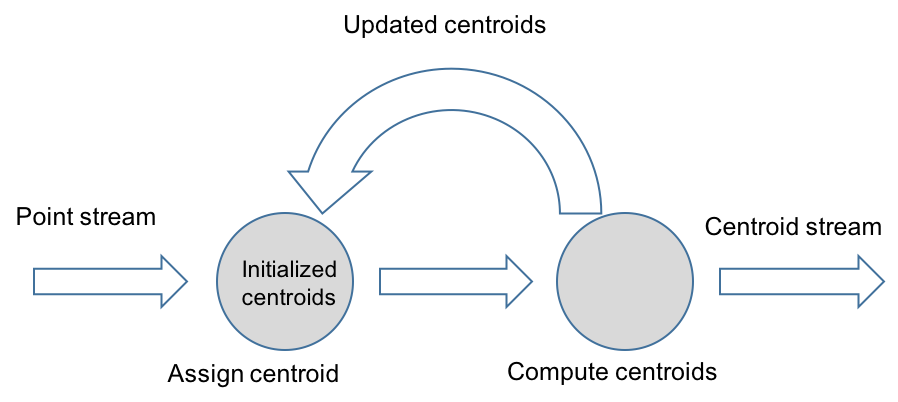
\includegraphics[scale=0.6]{images/iterator_operator}}
   \caption{Stream k-means scenario}
   \label{fig:iterator_operator}
  \end{center}
\end{figure}

Spark executes data analysis pipeline using directed acyclic graph scheduler.  Nested cycle doesn't exist in the data pipeline graph. Therefore, this workload will not be used to benchmark Spark Streaming. Instead, a standalone version of k-means application is used to evaluate the performance of Spark Streaming.

\section{Data Generators}
\label{section:data_generator}
 A data generator is a program that produces and sends unbounded records continuously to kafka cluster which are consumed by corresponding workload. For each workload, we designed one or several data generators with some configureable parameters which define the skew in record popularity, the size of records, and the distribution of data etc. These parameters could be changed to evaluate the performance of a system executing one workload on similar data streams with different properties. Users of StreamBench also could implement their own data generators to produce benchmarking data. Data generators are defined in a submodule of StreamBench project named \textit{generator}. The submodule could be compiled and packaged to get a jar file that could run on any node of our kafka cluster. 

\subsection{WordCount}
\label{subsection:wordcount_generator}

A data generator of workload WordCount produces unbounded lists of sentences, each sentence consists of several words. In StreamBench, we have implemented two versions of WordCount data generator. Each word in both generators is a 5-digit zero-padded string of a binary integer,  such as ``00001". The number of words in each sentence satisfies normal distribution with mean and sigma configured as \texttt{(10, 1)}. The difference between these two generators is the corresponding integers satisfy two different distributions: uniform distribution and zipfian distribution. Both uniform distribution and zipfian distribution have the same size -- 10000. Exponent of zipfian distribution is configured as 1. 

There are two different ways to run WordCount data generators to cooperate experiments of WordCount discussed in \cref{section:wordcount_experiment}. For Online WordCount, we start data generation after benchmark program and pass a parameter when starting generator to control the generation speed. For Offline model, we could either preload data to kafka cluster or make the generation speed much faster than the throughput of stream processing system executing WordCount workload.

\subsection{AdvClick}
\label{subsection:advclick_generator}

As discussed in Section~\ref{sub:join_operator}, workload AdvClick performs join operator on two streams: \texttt{shown advertisements} and \texttt{advertisement clicks}. Each record in  \texttt{shown advertisements} is a tuple consist of a universally unique identifier(\textbf{UUID}) and a timestamp. Each advertisement has a probability to be clicked, which is set to 0.3 in our experiments. Then the data generator could be a multi-threads application with main thread producing advertisements and sub-threads generating clicks. The pseudocode of the main thread is shown as Algorithm \ref{alg:advclick_generator}. After a sub-thread starts, it sleeps for delta time and then sends click record to corresponding kafka topic. The probability of advertisements click is a configureable parameter. In our experiments, mean of click delay is set to 10 seconds. 

\begin{algorithm}
\caption{AdvClick data generator}
\label{alg:advclick_generator}
\begin{algorithmic}[1]
\State $\text{load } \textit{clickProbability} \text{ from configure file}$

\State $\textit{cachedThreadPool} \gets \text{new CachedThreadPool}$
\State $\textit{dataGenerator} \gets \text{new RandomDataGenerator}$ 
\State $\textit{producer} \gets \text{new KafkaProducer}$ 

\While{not interrupted}
\State $\textit{advId} \gets \text{new UUID}$ 
\State $\textit{timestamp} \gets \text{current timestamp}$ 
\State $\textit{producer.send(...)}$ 

\If {$\textit{generator.nextUniform(0,1)} < clickProbability$} 
\State $\textit{deltaTime} \gets \textit{generator.nextGaussian(...)}$ 
\State $\textit{cachedPool.submit(new ClickThread(advId, daltaTime))} $ 
\EndIf
\EndWhile
\end{algorithmic}
\end{algorithm}

\subsection{KMeans}

Stream k-means is a one-pass clustering algorithm for stream data. In this workload, it is used to cluster a unbounded stream of points. The data generator produces such a stream of points. In order to make experiment results checking easy, we use pre-defined centroids. First, a set of centers are generated and written to a external file. There is a minimum distance between every two centers so that no two clusters are overlapped together. Then the generator produces points according these centers as Algorithm~\ref{alg:kmeans_generator}. The distance of each point to corresponding center satisfies normal distribution with mean and variance as configurable parameters. In our experiments, we found that random initial centroids would lead to results that two groups points cluster to a centroid which is in the middle of two real centers. Which is not desired output to measure the speed of convergence. Therefore, we generate initial centroids for each cluster in the same way as points generation.  

\begin{algorithm}
\caption{KMeans data generator}\label{euclid}
\label{alg:kmeans_generator}
\begin{algorithmic}[1]
\State $\text{load } \textit{covariances} \text{ from configure file}$
\State $\textit{means} \gets \text{original point}$
\State $\text{load } \textit{centroids} \text{ from external file}$

\State $\textit{producer} \gets \text{new KafkaProducer}$ 
\State $\textit{normalDistributon } \gets \text{ new NormalDistribution(means, converiances)}$

\While{not interrupted}
\State $\textit{centroid} \gets \text{pick a centroid from \textit{centroids} randomly}$ 
\State $\textit{point} \gets \textit{centroid+normalDistributon.sample()}$ 
\State $\textit{producer.send(point)}$ 

\EndWhile
\end{algorithmic}
\end{algorithm}

In our experiment environment, the compute cluster consists of 8 work nodes, each work node has 4 cpu cores. The parallelism of the compute cluster is 32. In order to have a better workload balance, we set the number of centers as 96. The dimension of point is configurable that enables to evaluate whether computation is a bottleneck of this workload.

\section{Experiment Logging and Statistic}
\label{section:log_statistic}

For evaluating the performance, there are two performance measurement terms used in StreamBench that are latency and throughput. Latency is the required time from a record entering the system to some results produced after some actions performed on the record. In StreamBench, messaging system and stream processing system are combined together and treated as one single system. The latency is computed start from when a record is generated. As discussed in Section \ref{section:data_generator}, data is sent to kafka cluster immediately after generation. Figure~\ref{fig:latency} shows how latency computed in StreamBench. In our experiments, we noticed that in the beginning of processing data, the performance of Storm cluster is bad. That leads to high latency of records in the head of a stream. Therefore, we ignored latency logs of first 1 minute in our statistic.

Throughput is the number of actions executed or results produced per unit of time. In the WordCount workload, throughput is computed as the number of words counted per seconds in the whole compute cluster. Joined click events and the number of points processed per second are the throughput of workloads AdvClick and Stream KMeans respectively.

There is an inherent tradeoff between latency and throughput: on a given hardware setup, as the amount of load increases by increase the speed of data generation, the latency of individual records increases as well since there is more contention for disk, CPU, network, and so on. Computing latency start from records generated makes it easy to measure the highest throughput, since records couldn't produced in time will stay in kafka topics that increase latency dramatically. A stream processing system with better performance will achieve low latency and high throughput with fewer servers.

\begin{figure}
  \begin{center}
  \subfigure{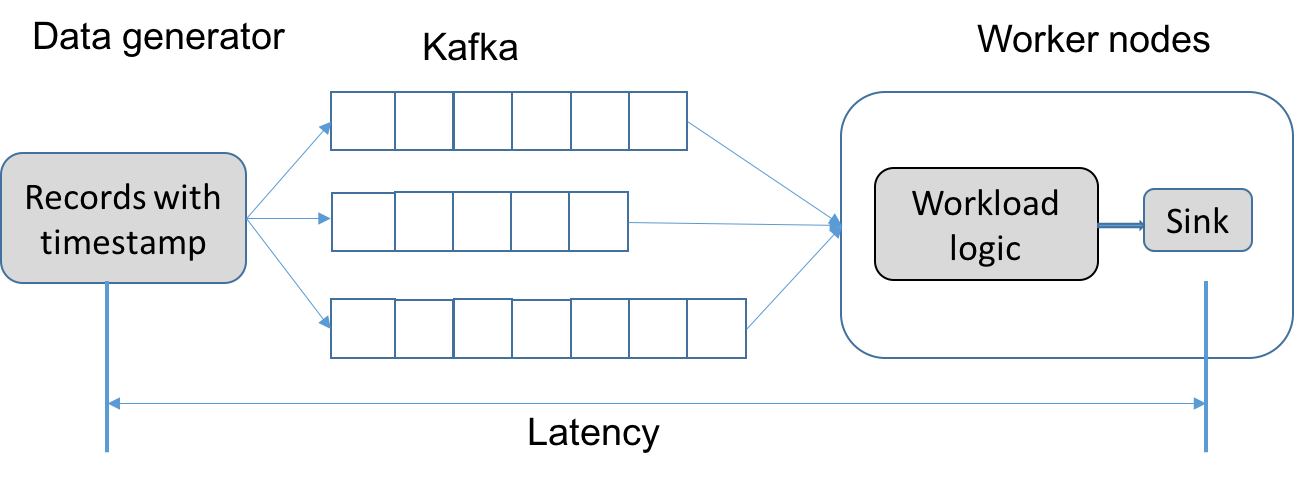
\includegraphics[scale=0.5]{images/latency}}
   \caption{Latency}
   \label{fig:latency}
  \end{center}
\end{figure}

\section{Extensibility}
\label{section:extensibility}

One significant feature of StreamBench is extensibility. The component "Workloads" in Figure~\ref{fig:streambench_architecture} contains three predefined workloads discussed in Section~\ref{section:workloads} that are implemented with common stream processing APIs. First, with some configuration modification of a data generator, which allows user to vary the skew in record popularity, and the size and number of records. The performances of a workload processing data streams with different properties could be different a lot. Moreover, it is easy for developers to design and implement a new workload to benchmark some specific features of stream processing systems. This approach allows for introducing more complex stream processing logic, and exploring tradeoffs of new stream processing features; but involves greater effort compared to the former approach.

Besides implementing new workloads, StreamBench also could be extended to benchmark new stream processing systems by implement a set of common stream processing APIs. A few samples of APIs could be shown as following:
\begin{itemize}
\item \textbf{map}(MapFunction\textless \textbf{T}, \textbf{R}\textgreater fun, String componentId): map each record in a stream from type \textbf{T} to type \textbf{R}
\item \textbf{mapToPair}(MapPairFunction\textless \textbf{T, K, V}\textgreater fun, String componentId): map a  item stream\textbf{\textless T\textgreater } to a pair stream\textbf{\textless K, V\textgreater}
\item \textbf{reduceByKey}(ReduceFunction\textless \textbf{V}\textgreater fun, String componentId): called on a pair stream of (\textbf{K, V}) pairs, return a new pair stream of (\textbf{K, V}) pairs where the values for each key are aggregated using the given reduce function
\end{itemize}

These methods are quite simple, representing common data transformations. There are some other APIs like \texttt{filter()}, \texttt{flatMap()} and \texttt{join} which are also easily to implement and supported well by most stream processing systems. Despite its simplicity, this API maps well to the native APIs of many of the stream processing systems we examined.





